\documentclass[11pt]{article}
\usepackage{multirow}
% Change "review" to "final" to generate the final (sometimes called camera-ready) version.
% Change to "preprint" to generate a non-anonymous version with page numbers.
\usepackage[review]{acl}

% Standard package includes
\usepackage{times}
\usepackage{latexsym}
\usepackage{booktabs}
\usepackage{float}
% For proper rendering and hyphenation of words containing Latin characters (including in bib files)
\usepackage[T1]{fontenc}
% For Vietnamese characters
% \usepackage[T5]{fontenc}
% See https://www.latex-project.org/help/documentation/encguide.pdf for other character sets

% This assumes your files are encoded as UTF8
\usepackage[utf8]{inputenc}

% This is not strictly necessary, and may be commented out,
% but it will improve the layout of the manuscript,
% and will typically save some space.
\usepackage{microtype}

% This is also not strictly necessary, and may be commented out.
% However, it will improve the aesthetics of text in
% the typewriter font.
\usepackage{inconsolata}
\usepackage{xcolor}
%Including images in your LaTeX document requires adding
%additional package(s)
\usepackage{graphicx}
\usepackage{amsmath}
\usepackage{amsthm}
\usepackage{amssymb}
\usepackage{enumitem}
\usepackage{pifont}
\usepackage{ulem}
\usepackage{algorithm}
\usepackage{algorithmic}

\theoremstyle{plain}
\newtheorem{proposition}{Proposition}[section]
\newtheorem{corollary}{Corollary}[proposition]
\theoremstyle{definition}
\newtheorem{definition}{Definition}[section]

\newcommand{\cmark}{\textcolor{green!60!black}{$\checkmark$}}
\newcommand{\xmark}{\textcolor{red}{$\times$}}
\newcommand{\Epub}{\mathcal{E}^{\mathrm{pub}}}
\newcommand{\Epriv}[1]{\mathcal{E}_{#1}^{\mathrm{priv}}}
\newcommand{\Eview}[1]{\mathcal{E}_{#1}}

% --- Case study styling ---
\usepackage{tcolorbox}
\tcbuselibrary{skins,breakable}
\usepackage{tabularx}

\definecolor{agA}{HTML}{1F4E79}
\definecolor{agB}{HTML}{B7472A}
\definecolor{agC}{HTML}{2E7D32}
\definecolor{okcol}{HTML}{2E7D32}
\definecolor{badcol}{HTML}{B71C1C}

\newcommand{\agA}[1]{\textcolor{agA}{\textbf{#1}}}
\newcommand{\agB}[1]{\textcolor{agB}{\textbf{#1}}}
\newcommand{\agC}[1]{\textcolor{agC}{\textbf{#1}}}
\newcolumntype{R}{>{\raggedright\arraybackslash}X}

% Success case (banner title wraps; checkmark icon)
\newtcolorbox{successcase}[1]{%
  enhanced, breakable,
  colback=okcol!3,
  colframe=okcol!50!black,
  arc=2pt, boxrule=0.5pt,
  title={\raggedright $\checkmark$\,\,#1},
  fonttitle=\bfseries\small,
  colbacktitle=okcol!55!black,
  coltitle=white,
  left=6pt, right=6pt, top=5pt, bottom=5pt,
  before skip=8pt, after skip=8pt,
}

% Failure case
\newtcolorbox{failurecase}[1]{%
  enhanced, breakable,
  colback=badcol!3,
  colframe=badcol!50!black,
  arc=2pt, boxrule=0.5pt,
  title={\raggedright $\times$\,\,#1},
  fonttitle=\bfseries\small,
  colbacktitle=badcol!55!black,
  coltitle=white,
  left=6pt, right=6pt, top=5pt, bottom=5pt,
  before skip=8pt, after skip=8pt,
}

% If the title and author information does not fit in the area allocated, uncomment the following
%
%\setlength\titlebox{<dim>}
%
% and set <dim> to something 5cm or larger.

\title{Diverse Evidence, Better Forecasts: Multi-Agent Deliberation Under Information Asymmetry}

% Author information can be set in various styles:
% For several authors from the same institution:
% \author{Author 1 \and ... \and Author n \\
%         Address line \\ ... \\ Address line}
% if the names do not fit well on one line use
%         Author 1 \\ {\bf Author 2} \\ ... \\ {\bf Author n} \\
% For authors from different institutions:
% \author{Author 1 \\ Address line \\  ... \\ Address line
%         \And  ... \And
%         Author n \\ Address line \\ ... \\ Address line}
% To start a separate ``row'' of authors use \AND, as in
% \author{Author 1 \\ Address line \\  ... \\ Address line
%         \AND
%         Author 2 \\ Address line \\ ... \\ Address line \And
%         Author 3 \\ Address line \\ ... \\ Address line}

\author{First Author \\
  Affiliation / Address line 1 \\
  Affiliation / Address line 2 \\
  Affiliation / Address line 3 \\
  \texttt{email@domain} \\\And
  Second Author \\
  Affiliation / Address line 1 \\
  Affiliation / Address line 2 \\
  Affiliation / Address line 3 \\
  \texttt{email@domain} \\}

%\author{
%  \textbf{First Author\textsuperscript{1}},
%  \textbf{Second Author\textsuperscript{1,2}},
%  \textbf{Third T. Author\textsuperscript{1}},
%  \textbf{Fourth Author\textsuperscript{1}},
%\\
%  \textbf{Fifth Author\textsuperscript{1,2}},
%  \textbf{Sixth Author\textsuperscript{1}},
%  \textbf{Seventh Author\textsuperscript{1}},
%  \textbf{Eighth Author \textsuperscript{1,2,3,4}},
%\\
%  \textbf{Ninth Author\textsuperscript{1}},
%  \textbf{Tenth Author\textsuperscript{1}},
%  \textbf{Eleventh E. Author\textsuperscript{1,2,3,4,5}},
%  \textbf{Twelfth Author\textsuperscript{1}},
%\\
%  \textbf{Thirteenth Author\textsuperscript{3}},
%  \textbf{Fourteenth F. Author\textsuperscript{2,4}},
%  \textbf{Fifteenth Author\textsuperscript{1}},
%  \textbf{Sixteenth Author\textsuperscript{1}},
%\\
%  \textbf{Seventeenth S. Author\textsuperscript{4,5}},
%  \textbf{Eighteenth Author\textsuperscript{3,4}},
%  \textbf{Nineteenth N. Author\textsuperscript{2,5}},
%  \textbf{Twentieth Author\textsuperscript{1}}
%\\
%\\
%  \textsuperscript{1}Affiliation 1,
%  \textsuperscript{2}Affiliation 2,
%  \textsuperscript{3}Affiliation 3,
%  \textsuperscript{4}Affiliation 4,
%  \textsuperscript{5}Affiliation 5
%\\
%  \small{
%    \textbf{Correspondence:} \href{mailto:email@domain}{email@domain}
%  }
%}

\begin{document}
\maketitle
\begin{abstract}
Multi-agent systems are increasingly used for forecasting future events, as deliberation among multiple LLMs is believed to improve reasoning and calibration. Yet existing approaches overlook a critical design choice: what information each agent receives.
When all agents are given identical evidence, deliberation collapses into herding rather than genuine belief revision, leaving multi-agent systems little better than a single agent. 
We identify this as a fundamental gap and propose \textit{designed information asymmetry} to close it: by partitioning evidence into shared public and disjoint private subsets, each agent holds exclusive knowledge that can only reach others through deliberation.
We theoretically show that this decomposition reduces inter-agent error correlation, and instantiate it in \textbf{InfoDelphi}, a framework combining relevance-aware evidence routing, rationale-based iterative deliberation, and confidence-weighted aggregation.
On \textsc{PolyGym}, a benchmark of 375 binary forecasting questions derived from real-world prediction markets, InfoDelphi outperforms the strongest single-agent and multi-agent baselines by 12--18\% in Brier score and 4--8 percentage points in accuracy.
More detailed experiments confirm that removing information asymmetry eliminates most deliberation gains, establishing diversity of input as the key enabler of effective multi-agent reasoning.
Our code is available at: \href{https://anonymous.4open.science/r/InfoDelphi}{Anonymous Repository}.
\end{abstract}

  % Large language models (LLMs) are increasingly applied to probabilistic
  % forecasting tasks, where a model must estimate the likelihood of real-world
  % events from retrieved textual evidence. Extending this paradigm to multi-agent
  % settings, where a panel of LLMs deliberates over shared predictions, is a
  % natural approach to improving forecast quality. However, existing multi-agent
  % pipelines suffer from a critical limitation: when agents are assigned
  % overlapping evidence, deliberation degenerates into reinforcement of the
  % majority view rather than genuine belief revision, a failure mode analogous
  % to herding in collective intelligence. This results in multi-round exchange
  % yielding little to no improvement over a single-agent baseline. We propose
  % a framework that addresses this by coupling relevance-aware evidence routing
  % with confidence-weighted aggregation. Specifically, we partition retrieved
  % documents using BM25 scores to construct complementary private views across
  % agents, ensuring information diversity as a prerequisite for effective
  % deliberation, and aggregate final-round forecasts by each agent's
  % self-reported confidence. On PolyGym, a dataset of 497 binary Polymarket
  % questions with temporally controlled evidence, our framework reduces Brier
  % score by 17.5\% and improves accuracy by 6.6 percentage points over a
  % single-agent RAG baseline. Ablation studies further confirm that evidence
  % routing is the load-bearing component: without it, iterative deliberation
  % provides no measurable benefit.

\section{Introduction}
\label{sec:intro}

Prediction markets such as Polymarket\footnote{\url{https://polymarket.com/}} aggregate the beliefs of thousands of participants into real-time probability estimates for future events, achieving forecasting
accuracy that often rivals or exceeds expert panels~\citep{tetlock2005expert}. With every question resolved against a definitive ground truth, these markets provide a natural benchmark for machine intelligence: \textit{\textbf{can an automated system reason over evidence and match human-level forecasting?}}

% Prediction markets such as Polymarket\footnote{\url{https://polymarket.com/}} aggregate the beliefs of thousands of participants into real-time probability estimates for future events.
% These markets have demonstrated forecasting accuracy that often rivals or exceeds expert panels~\citep{tetlock2005expert}, making them a natural benchmark for machine intelligence: \textit{\textbf{can an automated system reason over evidence and produce calibrated probabilistic forecasts at a human-competitive level?}}
Recent work has shown that large language models (LLMs) equipped with retrieved evidence can approach human-level performance on binary forecasting tasks~\citep{halawi2024approaching,turtel2025llms}, but these advances rely primarily on single-agent, single-pass pipelines that treat the entire evidence corpus as a monolithic context window.
A natural extension is the \textit{multi-agent} setting, where a panel of LLMs deliberates over the evidence before producing a collective forecast.
Such frameworks draw inspiration from well-studied human mechanisms for aggregating distributed knowledge---expert committees, structured interviews, and the Delphi method~\citep{DALKEY1969408}---and have shown promise in general reasoning tasks~\citep{chen2024reconcile,wangmixture}.

\vspace{-0.8em}

\begin{figure}[ht]
    \centering
    
\includegraphics[width=1\linewidth]{latex/intro.png}
    \caption{Effect of information asymmetry on a real prediction. \textbf{Left}: agents with identical evidence converge to the same incorrect forecast. \textbf{Right}: agents with complementary private evidence self-correct through rationale sharing, reducing Brier score from 0.45 to 0.004.}
    \label{fig:intro}
\end{figure}

\vspace{-0.8em}
Effective collective reasoning, however, requires that participants hold \textit{informationally diverse} views. As formalized in the Condorcet jury tradition and established empirically for human forecasters~\citep{Lorenz2011HowSI}, when agents share identical information, deliberation fails to improve collective accuracy: they reach the same conclusions independently, and iterative exchange merely reinforces the shared prior. In LLM systems this problem runs deeper. Recent work shows that models from different providers make correlated errors at rates above 60\%~\citep{kim2025correlated}, and that standard multi-agent debate under homogeneous input behaves as a \textit{martingale} whose expected accuracy does not improve over rounds~\citep{choi2026debate}.
Figure~\ref{fig:intro} illustrates this failure mode on a real prediction market question: when all agents receive identical evidence, they converge to the same incorrect forecast (left), whereas agents equipped with complementary private evidence can self-correct through deliberation (right).

To address this, we propose \textit{designed information asymmetry}, treating information asymmetry not as a limitation to overcome but as a principle to exploit.
We introduce \textbf{InfoDelphi}, a multi-agent forecasting framework that partitions evidence into a shared public pool and disjoint private subsets, giving each agent distinct expertise while preserving common ground for communication.
This mirrors effective human expert panels, where participants contribute complementary knowledge rather than reading the same briefing materials.
InfoDelphi constructs informative evidence partitions using BM25 relevance ranking.
During deliberation, agents exchange rationale excerpts rather than raw evidence, enabling efficient propagation of private signals.
Final forecasts are aggregated through confidence-weighted averaging in logit space, emphasizing the predictions of the best-informed agents.
Together, these design choices ensure that deliberation surfaces new information rather than reinforcing shared priors.

Furthermore, existing forecasting benchmarks entangle retrieval quality with reasoning ability, making it impossible to assess whether gains come from better search or better deliberation.
We introduce \textsc{PolyGym}, a controlled benchmark of 375 binary Polymarket questions with fixed, pre-retrieved evidence shared across all methods.
On \textsc{PolyGym}, InfoDelphi outperforms the strongest single-agent and multi-agent baselines by 12--18\% in Brier score and 4--8 percentage points in accuracy.
Detailed ablations confirm that the public/private split and rationale sharing are jointly necessary, as removing either eliminates most gains, and cross-model experiments demonstrate consistent improvements from open-source to frontier proprietary LLMs.
These results establish designed information asymmetry as a general principle for multi-agent reasoning under uncertainty.

Our main contributions are as follows:
\begin{itemize}[nosep,leftmargin=20pt,topsep=2pt,itemsep=1pt,parsep=0pt]
  \item We propose \textit{designed information asymmetry}  for multi-agent reasoning, and theoretically show that public/private evidence partitioning reduces inter-agent error correlation.
  
  \item We introduce \textbf{InfoDelphi}, which instantiates this principle through relevance-aware evidence routing, rationale-based deliberation, and confidence-weighted aggregation.
  
  \item We construct \textsc{PolyGym}, a controlled forecasting benchmark that isolates information utilization from retrieval, and conduct extensive experiments showing that (a) deliberation without information diversity provides little benefit, (b) rationale sharing is critical for cross-agent information transfer, and (c) gains generalize across different LLM backends.
\end{itemize}


\section{Related Work}
\label{sec:related}


\paragraph{LLM-based Forecasting.}
Early work established a substantial gap between LLM and human forecasting accuracy.
\citet{zou2022forecasting} find that language models achieve only 65\% accuracy on Autocast compared to 92\% for human aggregates, while \citet{schoenegger2023large} show that GPT-4 without augmentation does not significantly outperform a random baseline on Metaculus.
Retrieval-augmented generation~\citep{lewis2020retrieval} substantially closes this gap: \citet{yanautocast++} improve Autocast accuracy through zero-shot re-ranking and summarization of retrieved news, and \citet{halawi2024approaching} present a full pipeline achieving near-human performance on Polymarket and Metaculus.
More recent work focuses on training: \citet{turtel2025llms} fine-tune on 12,100 resolved Polymarket questions, and \citet{chandakscaling} train an 8B model via reinforcement
learning that matches proprietary LLMs on prediction benchmarks.
On the aggregation side, \citet{schoenegger2024wisdom} show that ensembling diverse
LLMs produces forecasts statistically indistinguishable from human forecasters.
Benchmark design has matured in parallel: ForecastBench~\citep{karger2024forecastbench}
and FutureX~\citep{zeng2025futurex} provide continuously updated evaluations with strict
temporal controls, and \citet{paleka2025pitfalls} identify systematic pitfalls including
temporal leakage and piggybacking on existing forecasts.
Despite this progress, existing pipelines treat forecasting as a single-agent process
and do not study evidence distribution across a deliberating panel.

\paragraph{Multi-Agent Reasoning and Deliberation.}
Multi-agent debate has emerged as a general strategy for improving LLM reasoning~\citep{du2023improving}.
\citet{wangself} show that sampling diverse chain-of-thought paths and selecting by majority vote improves accuracy, while \citet{wangmixture} propose Mixture-of-Agents, a layered architecture where later agents condition on all prior outputs.
\citet{chen2024reconcile} demonstrate that a round-table conference of diverse LLMs with confidence-weighted voting outperforms single-agent baselines across reasoning benchmarks.
However, recent theory suggests multi-agent debate is not uniformly beneficial.
\citet{choi2025debate} prove that under a Dirichlet-Categorical belief model, standard multi-agent debate forms a \textit{martingale}: expected correctness does not improve over rounds when agents receive identical inputs.
\citet{reasoningtrap2025} formalize this via the Data Processing Inequality: closed-system deliberation forms a Markov chain, so mutual information with the ground truth can only decrease.
\citet{kim2025correlated} document that LLM errors are 60\%+ correlated, implying that naive ensembling hits a non-zero error floor.
Our work addresses these limitations by introducing designed information asymmetry to break correlation and convert the martingale into productive belief revision.

\vspace{-0.5em}

\paragraph{Information Aggregation and Collective Intelligence.}
The conditions under which groups outperform individuals are well studied.
\citet{surowiecki2004wisdom} identify independence, diversity, and decentralized knowledge as key conditions for collective intelligence, while \citet{hong2004groups} show that diverse groups can outperform groups of only high-ability individuals.
The DeGroot model~\citep{612bb50a-4bdd-3a32-b6eb-7837600cc9c4} formalizes iterative belief aggregation, and the Delphi method~\citep{DALKEY1969408} applies structured multi-round elicitation to reduce expert disagreement.
For probabilistic forecasting, the linear opinion pool~\citep{9ca5e582-1e4c-323f-9ab1-c62032d22e48} and logit-space extremization~\citep{SATOPAA2014344} provide principled aggregation.
Meanwhile, social influence can suppress diversity without improving accuracy~\citep{Lorenz2011HowSI}, and informational cascades may cause agents to ignore private signals once consensus emerges~\citep{bikhchandani1992theory}.
Our framework operationalizes the positive conditions for collective intelligence while explicitly mitigating herding and information loss through evidence partitioning and rationale-based communication.

% =========================================================
\section{Methodology}
\label{sec:method}
% =========================================================

\subsection{Problem Formulation}

Let $q$ denote a binary forecasting question with resolution date $\tau$ and ground truth $y \in \{0,1\}$.
Each question is accompanied by a retrieved evidence corpus
$\mathcal{E} = \{e_1, \dots, e_n\}$, where $e_i$ consists of a title, URL, and textual snippet retrieved prior to $\tau$.
Therefore, given the question $q$ and evidence corpus $\mathcal{E}$, the goal is to estimate
$p(y = 1 \mid q, \mathcal{E})$,
where $p \in [0,1]$ denotes the predicted probability that the event resolves positively.


\subsection{Theoretical Motivation}
\label{sec:theory}

We begin by formalizing why information asymmetry improves collective forecasting, drawing on the bias-variance-covariance decomposition of the ensemble mean squared error.

\paragraph{Homogeneous input induces correlated errors.}
Consider $J$ agents each receiving the same evidence $\mathcal{E}$.
Let $p_j$ denote agent $j$'s forecast and $y$ the ground truth.
The ensemble forecast $\bar{p} = \frac{1}{J}\sum_j p_j$ has mean squared error:
\begin{equation}
  \mathrm{MSE}(\bar{p}) \;=\; \mathrm{Bias}^2 + \bar{\sigma}^2 - \mathrm{Div},
  \label{eq:bvd}
\end{equation}
where $\bar{\sigma}^2 = \frac{1}{J}\sum_j \mathrm{Var}(p_j)$ is the average agent variance and $\mathrm{Div} = \frac{1}{J}\sum_j \mathrm{Var}(p_j - \bar{p})$ is the diversity term~\citep{wood2023unified}.
When all agents observe identical input, their prediction errors $\epsilon_j = p_j - y$ are driven by the same evidence and thus highly correlated: $\mathrm{Cov}(\epsilon_i, \epsilon_j) \approx \mathrm{Var}(\epsilon)$ for $i \neq j$.
In this regime, the diversity term $\mathrm{Div}$ collapses toward zero, because agents conditioned on identical input produce nearly identical forecasts, and the ensemble provides no benefit over a single agent.
Recent empirical work confirms this: LLM errors are correlated across providers, and optimal aggregation under full correlation has a non-zero error floor~\citep{kim2025correlated,turkmen2026don}.

\paragraph{Information asymmetry reduces error correlation.}
We now show that the public/private evidence partition directly reduces this correlation.

\begin{proposition}[Diversity-Induced Decorrelation]
    \label{prop:decorrelation}
    Let each agent's prediction error decompose as
    $\epsilon_j = \rho \cdot \epsilon^{\mathrm{pub}} + (1-\rho) \cdot \epsilon_j^{\mathrm{priv}}$,
    where $\epsilon^{\mathrm{pub}}$ is the error component driven by shared public evidence,
    $\epsilon_j^{\mathrm{priv}}$ is the component driven by agent $j$'s private evidence,
    and $\rho \in [0,1]$ is the public ratio.
    Let $\sigma_{\mathrm{pub}}^2 = \mathrm{Var}(\epsilon^{\mathrm{pub}})$ and assume:
    \begin{enumerate}[label=(\roman*),nosep,leftmargin=20pt,topsep=2pt,itemsep=1pt]
    \item $\mathrm{Cov}(\epsilon_i^{\mathrm{priv}}, \epsilon_j^{\mathrm{priv}}) = 0$ for $i \neq j$ \textit{(private--private independence)};
    \item $\mathrm{Cov}(\epsilon^{\mathrm{pub}}, \epsilon_k^{\mathrm{priv}}) = 0$ for all $k$ \textit{(public--private independence)};
    \item $\mathrm{Var}(\epsilon_j^{\mathrm{priv}}) = \sigma_{\mathrm{priv}}^2$ for all $j$ \textit{(symmetric private noise)}.
  \end{enumerate}
    Then:
    \begin{equation}
      \mathrm{Corr}(\epsilon_i, \epsilon_j) \;=\;
      \frac{\rho^2\,\sigma_{\mathrm{pub}}^2}
           {\rho^2\,\sigma_{\mathrm{pub}}^2 + (1{-}\rho)^2\,\sigma_{\mathrm{priv}}^2}.
      \label{eq:corr}
    \end{equation}
  \end{proposition}

\begin{proof}
  By bilinearity of covariance and assumptions (i)--(ii), all cross-terms vanish,
  giving $\mathrm{Cov}(\epsilon_i, \epsilon_j) = \rho^2\sigma_{\mathrm{pub}}^2$.
  By assumptions (ii)--(iii), the cross-term in the variance expansion also vanishes,
  so $\mathrm{Var}(\epsilon_j) = \rho^2\sigma_{\mathrm{pub}}^2 + (1{-}\rho)^2\sigma_{\mathrm{priv}}^2$,
  which equals $\mathrm{Var}(\epsilon_i)$ by symmetry.
  Dividing covariance by $\sqrt{\mathrm{Var}(\epsilon_i)\mathrm{Var}(\epsilon_j)} = \mathrm{Var}(\epsilon_j)$
  gives~\eqref{eq:corr}.
  \end{proof}

  \noindent
  Proposition~\ref{prop:decorrelation} shows that inter-agent error correlation decreases
  monotonically as $\rho$ decreases from 1 to 0.
  As a concrete instance, at the default $\rho = 0.5$ with equal-variance components
  ($\sigma_{\mathrm{pub}} = \sigma_{\mathrm{priv}}$), correlation equals $0.25/(0.25+0.25) = 0.5$,
  half the all-public baseline ($\rho{=}1$, correlation~$= 1$).
  At $\rho = 0$ (all-private), agents are fully decorrelated; at $\rho = 1$ (all-public,
  standard debate), correlation reaches its maximum.

% \begin{proof}
% By decomposition, $\mathrm{Cov}(\epsilon_i, \epsilon_j) = \rho^2 \mathrm{Var}(\epsilon^{\mathrm{pub}})$ since the private components are independent.
% The individual variance is $\mathrm{Var}(\epsilon_j) = \rho^2 \mathrm{Var}(\epsilon^{\mathrm{pub}}) + (1-\rho)^2 \mathrm{Var}(\epsilon_j^{\mathrm{priv}})$. Dividing gives~\eqref{eq:corr}.
% \end{proof}

% \noindent
% Proposition~\ref{prop:decorrelation} shows that error correlation scales as $\rho^2$: halving the public ratio reduces inter-agent correlation by a factor of four.
% At $\rho = 0$ (all-private), the agents are fully decorrelated; at $\rho = 1$ (all-public, standard debate), the correlation reaches its maximum.


\begin{figure*}[!ht]
    \centering
    
\includegraphics[width=1\textwidth]{latex/framework.png}
  \caption{Overview of the \textbf{InfoDelphi} framework.
  (a)~\textbf{Evidence Routing}: documents are ranked by BM25 relevance and
  distributed round-robin, constructing a shared public pool and disjoint private
  subsets for each agent.
  (b)~\textbf{Multi-Agent Deliberation}: agents exchange structured forecasts and rationales over two rounds via a history summarizer, enabling private information to propagate.
  (c)~\textbf{Confidence-Weighted Aggregation}: final forecasts are combined by prediction-extremity weights ($w_j = |\mathrm{logit}(p_j)|$) into a single probability estimate.}
  \vspace{-1.5em}
    \label{fig:arch}
\end{figure*}


\begin{corollary}[Optimal Public Ratio Trade-off]
\label{cor:tradeoff}
Decreasing $\rho$ reduces error correlation (improving ensemble gain) but also reduces the shared context necessary for agents to interpret each other's rationales.
An optimal $\rho^* \in (0,1)$ therefore exists that balances diversity against communicability.
\end{corollary}

% Our ablation studies (Section~\ref{sec:ablation}) empirically identify $\rho^* = 0.5$ on \textsc{PolyGym}, consistent with this prediction.

\paragraph{Rationale sharing enables cross-agent information transfer.}
Even with disjoint evidence, agents cannot benefit from each other's private signals unless they communicate their \textit{reasoning}, not just their conclusions.
By the Data Processing Inequality~\citep{shin2026reasoning}, a deliberation system where agents only exchange numeric estimates forms a Markov chain $\mathcal{E}_j \to p_j^{(1)} \to p_j^{(2)} \to \cdots$, so $I(y; p_j^{(r+1)}) \leq I(y; p_j^{(r)})$: information with the ground truth can only decrease.
Sharing rationales breaks this Markov structure: agent $i$ now observes a summary of agent $j$'s reasoning over $\Epriv{j}$, effectively receiving a lossy projection of $j$'s private evidence.
This converts the system from closed to open, allowing $I(y; p_j^{(r+1)}) > I(y; p_j^{(r)})$, which is a necessary condition for iterative deliberation to improve over a single round.


% Our ablation confirms this: removing rationale sharing while retaining BM25 routing degrades Brier score by 0.033 (Table~\ref{tab:ablation}), the largest single degradation across all ablation dimensions. 



% \begin{definition}[Binary Forecasting]
% A \textit{forecast} is a probability estimate $\hat{p} \in [0,1]$ for the event $y=1$.
% Quality is measured by Brier score
% $\mathrm{BS} = \frac{1}{N}\sum_{k=1}^{N}(\hat{p}_k - y_k)^2$ (lower is better).
% \end{definition}

\subsection{The InfoDelphi Framework}

\paragraph{Overview.}

Figure~\ref{fig:arch} illustrates the end-to-end InfoDelphi pipeline.
Our theoretical analysis (Section~\ref{sec:theory}) identifies three conditions for effective collective forecasting: agents must hold \textit{diverse signals} (to reduce error correlation), share \textit{common ground} (to enable meaningful communication), and exchange \textit{reasoning} (to transfer private information).
InfoDelphi instantiates these conditions through three corresponding stages:
(1)~\textit{Evidence routing} partitions $\mathcal{E}$ into a shared public pool and disjoint private subsets via BM25 relevance ranking, simultaneously satisfying diversity and common ground;
(2)~\textit{Iterative deliberation} enables agents to exchange rationale excerpts across rounds, converting private signals into shared knowledge;
(3)~\textit{Confidence-weighted aggregation} combines final-round forecasts in logit space, amplifying agents whose private evidence supports stronger predictions.

\paragraph{Evidence Routing.}
\label{sec:routing}

We consider a panel of $J$ agents $\{A_1, \dots, A_J\}$ and a public ratio $\rho \in [0,1]$.
The corpus is partitioned into a shared public subset $\Epub$ and $J$ disjoint private subsets:
\begin{equation}
  \mathcal{E} \;=\; \Epub \;\cup\; \bigsqcup_{j=1}^{J} \Epriv{j},
  \ |\Epub| \;=\; \lfloor \rho \cdot |\mathcal{E}| \rfloor.
  \label{eq:partition}
\end{equation}
Agent $A_j$ observes the private view $\Eview{j} = \Epub \cup \Epriv{j}$.

To maximize information diversity across private subsets, we allocate documents via \textit{BM25 relevance routing}: each document $e_i \in \mathcal{E} \setminus \Epub$ receives a relevance score $s_i = \mathrm{BM25}(e_i, q)$.
The top-$|\Epub|$ scoring documents form $\Epub$: since these are the most directly relevant to the question, they serve as the shared ``language'' through which agents can interpret each other's reasoning during deliberation.
The remaining documents are sorted by $s_i$ and assigned to agents in round-robin order, so that adjacent relevance levels are spread across distinct private views.
This design ensures that each agent holds a unique slice of peripheral evidence while sharing access to core information, enabling diversity without sacrificing common ground.

\paragraph{Iterative Deliberation with Rationale Sharing.}
  \label{sec:deliberation}
 
  At each round $r \in \{1, \dots, R\}$, agent $A_j$ produces a structured forecast:
  \begin{equation}
    f_j^{(r)} \;=\; \bigl(p_j^{(r)},\, \ell_j^{(r)},\, r_j^{(r)}\bigr),
  \end{equation}
  where $p_j^{(r)} \in [0,1]$ is a probability estimate, $\ell_j^{(r)} \in \{0,1\}$ is a categorical prediction, and $r_j^{(r)}$ is a free-text
  rationale.
  The agent conditions on its private view and a history summary of prior-round forecasts:
  \begin{equation}
    f_j^{(r)} \;\sim\; \mathrm{LLM}\!\left(q,\;\Eview{j},\;h^{(r-1)}\right),
    \label{eq:agent}
  \end{equation}
  where $h^{(0)} = \varnothing$ and, for $r \geq 2$:
  \begin{equation}
    h^{(r-1)} \;=\; \bigl\{(p_k^{(r-1)},\,\ell_k^{(r-1)},\,r_k^{(r-1)})\bigr\}_{k \neq j}.
    \label{eq:history}
  \end{equation}
  Crucially, $h^{(r-1)}$ includes rationale excerpts from other agents, not only their numeric estimates.
  As established in Section~\ref{sec:theory}, this is what allows private evidence to propagate across agent boundaries.

  We study two deliberation protocols: \textit{independent forecasting},
  where agents reason solely from their private view; and \textit{iterative deliberation} (the full InfoDelphi protocol), where agents additionally
  observe all other agents' Round 1 forecasts and rationales before producing their final prediction.
  
  \paragraph{Confidence-Weighted Aggregation.}
  \label{sec:aggregation}

  Given $J$ agents' final-round forecasts $\{f_j^{(R)}\}_{j=1}^{J}$, we aggregate them via \textit{Confidence-Weighted (CW) pooling}:
  \begin{align}
    \hat{p}_{\mathrm{CW}} &\;=\; \sigma\!\left(
      \frac{\displaystyle\sum_{j=1}^{J} w_j \cdot \mathrm{logit}(p_j^{(R)})}
           {\displaystyle\sum_{j=1}^{J} w_j}
    \right), \nonumber\\
    w_j &= \bigl|\mathrm{logit}(p_j^{(R)})\bigr|
    \label{eq:cw}
  \end{align}
  where $\sigma(\cdot)$ is the sigmoid function and $w_j = |\mathrm{logit}(p_j^{(R)})|$ weights each agent by the extremity of its prediction.
Aggregation is performed in logit space to respect bounded probabilities. This is equivalent to weighted geometric averaging of odds ratios and coincides with the logarithmic opinion pool under uniform weights~\citep{10.1214/ss/1177013825}.
Agents with stronger private evidence produce more extreme forecasts, so up-weighting them amplifies the most informed signals.
  % Aggregation is performed in logit space to respect the bounded nature of probabilities; this is equivalent to weighted geometric averaging of odds
  % ratios, which coincides with the logarithmic opinion pool when weights are uniform~\citep{10.1214/ss/1177013825}.
  % The intuition is that agents with stronger private evidence tend to produce more extreme forecasts;
  % up-weighting such agents therefore amplifies the most informed signals in the final prediction.
% ---a property we verify empirically in Section~\ref{sec:analysis}.

% The design intuition is grounded in our empirical finding (Section~\ref{sec:analysis}) that prediction extremity strongly predicts accuracy: agents who assign probabilities far from 0.5 are substantially more accurate, validating the use of confidence as a proxy for evidence quality.

% =========================================================
\vspace{-0.8em}
\section{Experimental Setup}
\label{sec:setup}
\vspace{-0.5em}
% =========================================================

\paragraph{Dataset.}
Current LLM forecasting systems~\citep{halawi2024approaching,turtel2025llms} primarily emphasize \textit{retrieval quality}, while an equally important capability is \textit{information utilization}: how agents interpret, distribute, and collaboratively reason over retrieved evidence.
To study this dimension in isolation, we construct \textbf{\textsc{PolyGym}}, a controlled forecasting benchmark built from real-world Polymarket questions.
Specifically, \textsc{PolyGym} contains 375 binary forecasting markets with temporally filtered evidence corpora, where each question is paired with up to 30 pre-retrieved documents collected before market resolution.
Unlike live forecasting benchmarks, all methods operate over the same fixed evidence pool, eliminating variability from changing web environments and unstable search results.
This design enables reproducible evaluation of multi-agent deliberation strategies under controlled information conditions.
Importantly, \textsc{PolyGym} explicitly supports the study of \textit{designed information asymmetry}, as it isolates whether performance gains arise from improved reasoning and coordination rather than from superior retrieval alone.
More details in Appendix~\ref{sec:appendix_dataset}.

\paragraph{Baselines.}
We compare against two categories of baselines (details in Appendix~\ref{sec:appendix_details}).
\ding{182} \textit{Single-agent methods}: Zero-shot~\citep{kojima2022large}, Sequential Bayesian~\citep{shi2023language}, Chain-of-Thought~\citep{wei2022chain}, Self-Consistency~\citep{wangself}, Halawi et al.~\citep{halawi2024approaching}, and Superforecaster~\citep{karger2024forecastbench}.
\ding{183} \textit{Multi-agent methods with homogeneous input}: Standard Debate~\citep{du2023improving}, MoA~\citep{wangmixture}, Crowd Ensemble~\citep{schoenegger2024wisdom}, and AIA Forecaster~\citep{alur2025aia}.

\paragraph{Metrics.}
We report two complementary metrics.
The \textit{Brier score} $\mathrm{BS} = \frac{1}{N}\sum_{k=1}^{N}(\hat{p}_k - y_k)^2$ measures probabilistic calibration.
\textit{Accuracy} reports the fraction of questions for which the predicted label $\mathbf{1}[\hat{p} \geq 0.5]$ matches the ground-truth $y$.

\paragraph{Implementation.}
All experiments use \texttt{gpt-5.4-mini} via the OpenRouter API\footnote{\href{https://openrouter.ai/}{openrouter.ai}} as the primary model.
We use $J=3$ agents, $R=2$ deliberation rounds, and $\rho=0.5$ as default settings, with temperature 0.7, random seed 42, and parallelization across 15 workers.

% =========================================================
\section{Results}
\label{sec:results}
% =========================================================

\subsection{Main Results}

Table~\ref{tab:main} compares InfoDelphi under independent and iterative deliberation protocols with baselines.

\paragraph{\ding{224} Overall performance.}
InfoDelphi achieves the best Brier score (0.178) and accuracy (77.9\%) across all methods.
The improvement stems from two complementary mechanisms: \uline{information partitioning} creates diverse signals that reduce correlated errors, and \uline{rationale-based deliberation} allows agents to correct each other using their private evidence.
Notably, even without deliberation ($R{=}1$), InfoDelphi already achieves the second-highest accuracy (74.1\%), confirming that the diversity introduced by evidence routing provides value \textit{before} any inter-agent communication occurs.
Deliberation then amplifies this by enabling agents to propagate their private insights to others.

\begin{table}[ht]
\centering
\caption{Results on \textsc{PolyGym} ($N=375$). Methods are grouped by category. \textbf{Bold} is the best; \underline{underline} is the second best.}

\label{tab:main}
\resizebox{\columnwidth}{!}{
\begin{tabular}{llcc}
\toprule
\textbf{Category} & \textbf{Method} & \textbf{Brier}$\downarrow$ & \textbf{Acc}$\uparrow$ \\
\midrule
\multirow{6}{*}{\rotatebox{90}{\small Single-Agent}}
 & Zero-shot~\citep{kojima2022large} & \underline{0.201} & 66.7\% \\
 % & Direct & 0.227 & 70.7\% \\
 & Seq.\ Bayesian~\citep{shi2023language} & 0.256 & 62.1\% \\
 & Chain-of-Thought~\citep{wei2022chain} & 0.216 & 69.9\% \\
 & Self-Consistency~\citep{wangself} & 0.221 & 69.6\% \\
 & Halawi et al.~\citep{halawi2024approaching} & 0.238 & 65.3\% \\
 & Superforecaster~\citep{karger2024forecastbench} & 0.242 & 68.8\% \\
\midrule
\multirow{4}{*}{\rotatebox{90}{\small Multi-Agent}}
 & Standard Debate~\citep{du2023improving} & 0.202 & 73.9\% \\
 & MoA~\citep{wangmixture} & 0.220 & 70.9\% \\
 & Crowd Ensemble~\citep{schoenegger2024wisdom} & 0.245 & 65.9\% \\
 & AIA Forecaster~\citep{alur2025aia} & 0.247 & 67.7\% \\
\midrule
\multirow{2}{*}{\rotatebox{90}{\small Ours}}
 & InfoDelphi (no deliberation) & 0.206 & \underline{74.1\%} \\
 & \textbf{InfoDelphi} & \textbf{0.178} & \textbf{77.9\%} \\
\bottomrule
\end{tabular}
}
\vspace{-1em}
\end{table}

\paragraph{\ding{224} Information diversity is the key enabler.}
Across all baselines, neither scaling the number of agents, improving prompting strategies, nor adding sophisticated aggregation mechanisms yields meaningful gains without information diversity.
Multi-agent methods with homogeneous input (MoA, Crowd Ensemble, AIA Forecaster) fail to outperform a single Chain-of-Thought agent despite deploying 3--10 agents with various aggregation strategies.
Similarly, single-agent methods with elaborate prompting (Halawi's 7-step scratchpad, Superforecaster's structured reasoning) perform \textit{worse} than simple Chain-of-Thought, suggesting that more elaborate reasoning on noisy evidence amplifies rather than mitigates errors.
The one partial exception is Standard Debate, which benefits from iterative belief revision, yet it remains well below InfoDelphi because agents sharing identical evidence can only reinforce existing interpretations rather than introduce genuinely new perspectives.
These results are consistent with the prediction of Proposition~\ref{prop:decorrelation}: without information asymmetry, inter-agent error correlation remains high and aggregation provides diminishing returns.

\subsection{Ablation Studies}
\label{sec:ablation}

We ablate each design dimension against the default InfoDelphi configuration
($J{=}3$ agents, $R{=}2$ rounds, $\rho{=}0.5$, BM25 routing, confidence-weighted aggregation, with rationale sharing).
Each ablation varies one component while holding others fixed (detailed settings are provided in Appendix~\ref{sec:appendix_details}).

\begin{table}[ht]
\centering
\caption{Ablation results on \textsc{PolyGym}. Each row varies one component from the default InfoDelphi configuration. \textbf{Bold} is the best.}

\label{tab:ablation}
\resizebox{\columnwidth}{!}{
\begin{tabular}{llcc}
\toprule
\textbf{Dimension} & \textbf{Setting} & \textbf{Brier}$\downarrow$ & \textbf{Acc}$\uparrow$ \\
\midrule
\multirow{3}{*}{Rounds}
  & $R{=}1$ (no deliberation) & 0.206 & 74.1\% \\
  & $R{=}2$ (default) & \textbf{0.178} & \textbf{77.9\%} \\
  & $R{=}3$ & 0.196 & 75.7\% \\
\midrule
\multirow{3}{*}{Public ratio}
  & $\rho{=}0.3$ & 0.191 & 75.5\% \\
  & $\rho{=}0.5$ (default) & \textbf{0.178} & \textbf{77.9\%} \\
  & $\rho{=}1.0$ (all public) & 0.193 & 75.7\% \\
\midrule
\multirow{2}{*}{Rationale sharing}
  & Without & 0.211 & 70.4\% \\
  & With (default) & \textbf{0.178} & \textbf{77.9\%} \\
\midrule
\multirow{2}{*}{Aggregation}
  & Uniform weighting & 0.196 & 74.9\% \\
  & Confidence-weighted (default) & \textbf{0.178} & \textbf{77.9\%} \\
\midrule
\multirow{2}{*}{Evidence routing}
  & Random allocation & 0.188 & 76.2\% \\
  & Relevance-based (default) & \textbf{0.178} & \textbf{77.9\%} \\
\bottomrule
\end{tabular}
}
\vspace{-1em}
\end{table}

\paragraph{\ding{224} Creating asymmetry is necessary but not sufficient.}
Section~\ref{sec:theory} argues that effective collective reasoning requires three conditions: diverse signals, common ground, and reasoning exchange.
The ablation results confirm this hierarchy.
Simply partitioning evidence without deliberation already outperforms most homogeneous baselines; adding a second round yields a further $-$0.028 Brier reduction, demonstrating that information asymmetry creates the \textit{potential} for improvement while deliberation \textit{realizes} it.
However, a third round reverses this gain: with a finite evidence pool, two rounds suffice to propagate most private signals, and further deliberation leads to convergence toward a group consensus rather than continued refinement.

\paragraph{\ding{224} How agents communicate determines whether deliberation helps.}
The largest degradation occurs when rationale sharing is removed, reducing deliberation to a closed system.
This validates the DPI argument: exchanging only numeric estimates preserves the Markov structure and prevents private information from flowing across agent boundaries.
With rationale sharing, agents receive a lossy projection of each other's private evidence; without it, information about ground truth can only decrease over rounds.

\paragraph{\ding{224} The balance between diversity and common ground.}
The public ratio $\rho$ reveals an asymmetric failure mode: too little shared context ($\rho{=}0.3$) is as harmful as too much ($\rho{=}1.0$), but for different reasons. The former breaks communication while the latter eliminates diversity.
Even at the optimal split ($\rho{=}0.5$), the \textit{method} of allocation still matters: relevance-based routing outperforms random by 0.010 Brier.
This suggests that effective information asymmetry is not just about \textit{how much} to split, but about ensuring the public pool serves as meaningful common ground while private subsets contain genuinely complementary signals.

\paragraph{\ding{224} Confidence-weighted aggregation amplifies informed agents.}
Replacing confidence-weighted aggregation with uniform weighting degrades Brier by 0.018, showing that not all agents contribute equally after deliberation.
Agents with stronger private evidence produce more extreme predictions, and up-weighting them concentrates influence in the most informed voices (validated in Section~\ref{sec:analysis}).

\paragraph{\ding{224} Summary.}
The ablations reveal that InfoDelphi's gains are driven by the \textit{principle} of designed information asymmetry rather than any single algorithmic component.
Rationale sharing and the public/private split are the load-bearing design choices, while the routing algorithm and aggregation scheme provide further gains but are not irreplaceable, implying that the framework generalizes beyond its current form: alternative evidence partitioning strategies (e.g., dense retrieval) or aggregation methods can be substituted while preserving the benefit of information-diverse deliberation.

\subsection{Cross-Model Generalization}
\label{sec:crossmodel}

\newcommand{\micon}[1]{\raisebox{-1pt}{\includegraphics[height=9pt]{#1}}}
\newcommand{\mname}[2]{\micon{#1}\hspace{2pt}{#2}}

\begin{table}[t]
\centering
\caption{Cross-model generalization of InfoDelphi (mean $\pm$ std over 3 runs).}
\label{tab:crossmodel}
\small
\resizebox{\columnwidth}{!}{
\begin{tabular}{lcccc}
\toprule
 & \multicolumn{2}{c}{\textbf{Independent}} & \multicolumn{2}{c}{\textbf{Iterative}} \\
\cmidrule(lr){2-3}\cmidrule(lr){4-5}
\textbf{Model} & Brier$\downarrow$ & Acc$\uparrow$ & Brier$\downarrow$ & Acc$\uparrow$ \\
\midrule
\mname{latex/logo/meta.png}{Llama-4-Scout} & .209\tiny{$\pm$.002} & 67.3\tiny{$\pm$0.7}\% & .204\tiny{$\pm$.002} & 68.3\tiny{$\pm$0.6}\% \\
\mname{latex/logo/openai.pdf}{GPT-5.4-mini} & .208\tiny{$\pm$.005} & 73.8\tiny{$\pm$0.8}\% & .189\tiny{$\pm$.009} & 76.7\tiny{$\pm$1.2}\% \\
\mname{latex/logo/deepseek.png}{DeepSeek-V3.2} & .184\tiny{$\pm$.001} & 75.4\tiny{$\pm$0.9}\% & \textbf{.163}\tiny{$\pm$.005} & \textbf{79.6}\tiny{$\pm$1.3}\% \\
\bottomrule
\end{tabular}
}
\vspace{-1em}
\end{table}

To verify that InfoDelphi's gains are not specific to a single model, we evaluate the full framework on additional backends: DeepSeek-V3.2~\citep{liu2025deepseek} and Llama-4-Scout-17B~\citep{adcock2026llama}, as shown in Table~\ref{tab:crossmodel}.
All three models benefit from iterative deliberation, with the gain scaling with model capability.
This pattern suggests that stronger models extract more value from rationale sharing, as interpreting others' reasoning requires sufficient comprehension ability.
Notably, even the smallest model benefits from information partitioning alone (its independent mode already outperforms homogeneous multi-agent baselines), confirming that the framework is effective across the full spectrum of model capabilities.

\subsection{Detailed Analysis}
\label{sec:analysis}

\paragraph{\ding{224} Why does confidence weighting work in the asymmetric setting?}
Our confidence-weighted aggregation rests on the assumption that agents with stronger private evidence will produce more extreme predictions.
Figure~\ref{fig:extremity} validates this: accuracy increases monotonically from 62.7\% in the least extreme quartile to 94.7\% in the most extreme, while Brier score falls from 0.235 to 0.052.
However, a deeper question is why CW works \textit{better under information asymmetry} than under homogeneous input.
We find that individual agents are equally extreme in both settings (mean $|p - 0.5| \approx 0.36$), but their predictions point in \textit{different directions} under InfoDelphi: inter-agent variance is 1.7$\times$ higher than in the homogeneous setting.
In other words, information asymmetry does not make agents more confident---it makes them confident about \textit{different things}.
CW aggregation therefore synthesizes diverse high-confidence signals grounded in complementary evidence, rather than merely amplifying a shared bias.

\begin{figure}[t]
  \centering
  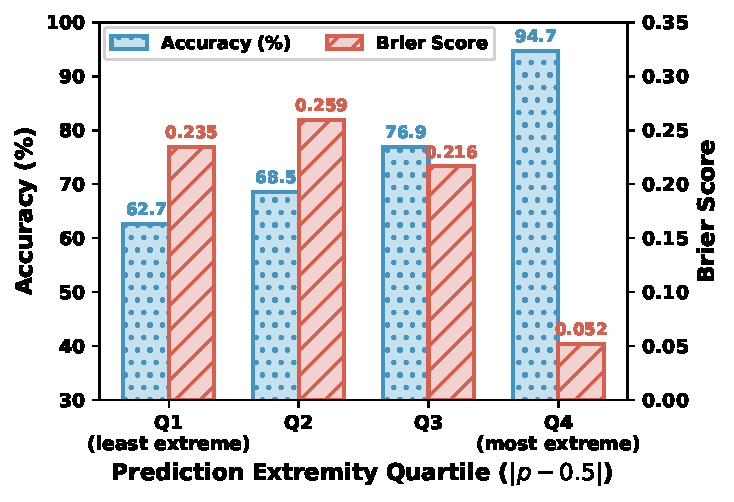
\includegraphics[width=\linewidth]{fig1_extremity_accuracy.pdf}
  \vspace{-2em}
  \caption{Accuracy and Brier score by prediction extremity quartile
    ($|p - 0.5|$). More extreme predictions correlate strongly with higher accuracy,
    validating the confidence-weighted aggregation design.}
  \label{fig:extremity}
  \vspace{-1.5em}
\end{figure}

\vspace{-0.5em}
\paragraph{\ding{224} Information asymmetry preserves diversity through deliberation.}
A key concern with iterative deliberation is herding: agents may converge toward a consensus regardless of their private evidence, collapsing the diversity that makes multi-agent systems valuable.
Figure~\ref{fig:variance} quantifies this by measuring inter-agent prediction variance before and after deliberation under three evidence allocation strategies.
Under All Info ($\rho{=}1.0$) and Random Split ($\rho{=}0.5$), deliberation reduces variance by 90--92\%, indicating near-complete convergence.
Under relevance-based routing ($\rho{=}0.5$), variance reduction is only 73\%, preserving substantially more inter-agent diversity.
This confirms that information asymmetry acts as a structural safeguard against herding: agents holding private evidence that they judge to be strongly predictive maintain distinct perspectives even after observing others' reasoning, because their exclusive information provides an independent basis for conviction that social pressure alone cannot override.

\begin{figure}[t]
  \centering
  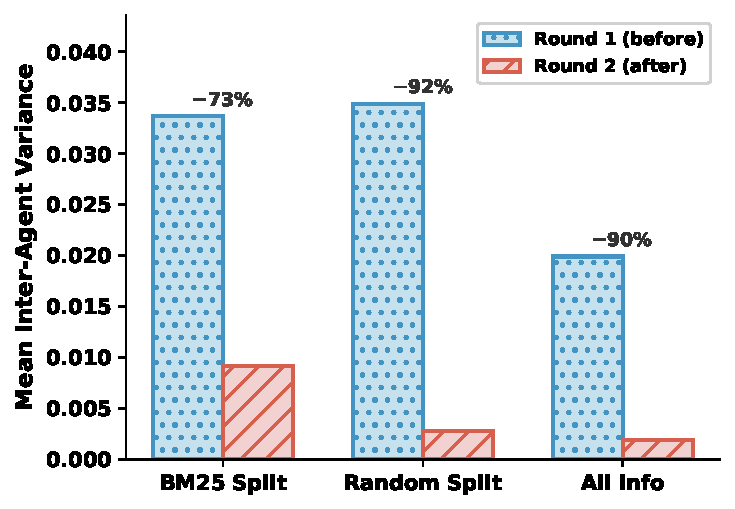
\includegraphics[width=\linewidth]{fig2_agent_variance.pdf}
  \vspace{-2em}
  \caption{Mean inter-agent prediction variance before (Round 1) and after (Round 2) deliberation. BM25 routing preserves substantially more diversity (73\% reduction) compared to Random Split and All Info.}
  \label{fig:variance}
    \vspace{-1em}
\end{figure}

\paragraph{\ding{224} Statistical significance.}
We verify that InfoDelphi's improvements are statistically significant via paired Wilcoxon signed-rank tests on per-question Brier scores (Table~\ref{tab:significance}).
InfoDelphi significantly outperforms all baselines ($p < 0.05$), with the strongest significance against methods that scale agents without information diversity (Crowd Ensemble, AIA Forecaster: $p < 0.001$).
Bootstrap 95\% confidence interval for InfoDelphi's Brier score is [0.147, 0.212], non-overlapping with Single-Agent's [0.185, 0.249].

\begin{table}[t]
\centering
\caption{Statistical significance of InfoDelphi vs.\ baselines (paired Wilcoxon signed-rank test).}
\label{tab:significance}
\small
\begin{tabular}{lcc}
\toprule
\textbf{Baseline} & $\Delta$\textbf{Brier} & \textbf{p-value} \\
\midrule
vs.\ Single-Agent & $-$0.038 & $<$0.001 \\
vs.\ Standard Debate & $-$0.023 & 0.021 \\
vs.\ MoA & $-$0.042 & 0.010 \\
vs.\ Crowd Ensemble & $-$0.067 & $<$0.001 \\
vs.\ AIA Forecaster & $-$0.069 & $<$0.001 \\
\bottomrule
\end{tabular}
\vspace{-1em}
\end{table}

% \paragraph{\ding{224} Error analysis.}
% Comparing InfoDelphi against the Single-Agent baseline at the question level: InfoDelphi uniquely corrects 58 questions that Single-Agent gets wrong, while regressing on 28 (net gain: +30 questions).
% Examining the 28 regression cases reveals a consistent pattern: evidence contains outdated price data (e.g., BTC at \$71K from an earlier snapshot) that contradicts the actual resolution (BTC above \$96K).
% Since all agents receive subsets of the same evidence corpus, information asymmetry cannot correct for evidence that is \textit{uniformly} misleading.
% In contrast, the 58 success cases show a different pattern: Single-Agent is overwhelmed by a dominant but incorrect signal in the evidence, while InfoDelphi's private-evidence routing ensures at least one agent encounters a contradicting signal that, through rationale sharing, corrects the group.

% =========================================================
\section{Conclusion}
\label{sec:conclusion}
% =========================================================
We presented \textbf{InfoDelphi}, a multi-agent forecasting framework built on a simple but overlooked insight: collective reasoning only outperforms individual reasoning when participants hold genuinely different information.
By treating information asymmetry as a first-class design principle, InfoDelphi converts redundant deliberation into productive belief revision, achieving consistent gains across model scales and families on \textsc{PolyGym}.
Probabilistic forecasting represents a particularly demanding test of this principle, requiring synthesis of noisy, contradictory evidence into calibrated estimates under irreducible uncertainty.
That designed information asymmetry yields robust improvements in this setting suggests broad applicability to multi-agent systems where agents reason over shared evidence, from collaborative question answering to scientific hypothesis evaluation to complex decision support.
  
\section*{Limitations}

  \paragraph{Theoretical assumptions.}
  Proposition~\ref{prop:decorrelation} rests on three idealizing assumptions:  a linear error decomposition, public--private independence, and symmetric private noise. In practice, documents retrieved for the same question share topical correlations,
  partially violating the independence assumptions and making the decorrelation bound
  approximate. The linear decomposition further assumes that public and private error components
  combine with fixed weights $\rho$ and $1{-}\rho$, a functional form that LLMs,
  as non-linear functions of their inputs, need not satisfy.

  % \paragraph{Model homogeneity.}
  % All agents in our primary experiments share the same underlying LLM, so errors remain correlated at the model level regardless of evidence partitioning.
  % Designed information asymmetry reduces \textit{evidence-driven} correlation but cannot eliminate \textit{model-level} correlation.

  % \paragraph{Confidence proxy.}
  % Confidence-weighted aggregation assumes that self-reported confidence correlates with forecast accuracy.
  % While Figure~\ref{fig:extremity} confirms this correlation empirically in our setting, the reliability of prediction extremity as a confidence proxy
  % may vary across question types and model families.

  \paragraph{Scope.}
  API cost scales linearly with agents $\times$ rounds (${\sim}\$12$ for 375 questions), which limits our ability to conduct large-scale experiments with more agents or deliberation rounds that would be needed to precisely characterize convergence behavior.
  Additionally, as our primary contribution is the multi-agent paradigm of designed information asymmetry, both evidence routing (BM25) and aggregation (confidence-weighted pooling) employ standard off-the-shelf methods; more sophisticated alternatives may yield further gains.

\section*{Ethics Statement}
  This work presents a forecasting framework and does not directly enable disinformation or harm beyond risks inherent to LLM-based systems generally. However, automated probability estimates generated at scale could in principle be misused to manipulate market sentiment or create false impressions of consensus. We recommend that InfoDelphi be used as a decision-support tool with human oversight in high-stakes deployment contexts.
% Bibliography
\bibliography{custom}

\appendix

\section{Discussion}
\paragraph{Key insight.}
Our central finding is that \textit{designed information asymmetry} is necessary for effective multi-agent deliberation.
When all agents receive identical evidence, iterative discussion provides little measurable benefit, as agents merely reinforce correlated beliefs rather than contribute complementary knowledge.
This aligns with the martingale characterization of homogeneous-input debate and suggests that the widely adopted practice of giving all agents the same context fundamentally limits the value of multi-agent interaction.

% \paragraph{Limitations.}
% (1)~Proposition~\ref{prop:decorrelation} relies on a linear error decomposition; LLMs
% are non-linear, so the bound is approximate in practice.
% (2)~Evaluation is limited to binary forecasting on a single benchmark.
% (3)~Evidence is static; live retrieval may introduce additional dynamics.
% (4)~Cost scales linearly with agents $\times$ rounds (${\sim}\$7{-}9$ for 375 questions
% in the default configuration).

  \paragraph{Future work.}
Natural extensions include (1)~adaptive routing that dynamically adjusts evidence allocation based on emerging disagreement, (2)~more expressive routing algorithms beyond BM25, such as dense retrieval or learned semantic partitioning, (3)~learned aggregation weights replacing self-reported confidence, (4)~evaluation on open-ended and multi-choice forecasting tasks, and (5)~heterogeneous model panels that leverage model-level diversity in addition to evidence-level asymmetry.



\paragraph{Potential Risks.}
Designed information asymmetry encourages agents to maintain distinct beliefs, but it may also amplify biased or misleading evidence partitions. If private evidence subsets contain low-quality, adversarial, or outdated documents, agents may become confidently polarized around incorrect conclusions rather than self-correcting through deliberation. In high-stakes domains such as finance or geopolitics, this could reinforce speculative narratives or misleading impressions of certainty. In addition, rationale sharing introduces a potential attack surface, where persuasive but flawed rationales propagate errors across agents. Future deployments should therefore incorporate evidence verification, source reliability estimation, and safeguards against adversarial persuasion.

\section{\textbf{\textsc{PolyGym}} Benchmark Details}
\label{sec:appendix_dataset}

\paragraph{Motivation.}
Agentic forecasting systems for prediction markets require two distinct capabilities:
(1)~\textit{retrieval}, identifying relevant information from the web, and
(2)~\textit{utilization}, reasoning over that information to produce calibrated probability estimates.
Existing benchmarks predominantly evaluate these capabilities jointly (Table~\ref{tab:benchmark_comparison}),
making it difficult to determine whether performance gains arise from better retrieval or better collective reasoning.
Also, live benchmarks~\citep{karger2024forecastbench,zeng2025futurex} introduce variability from changing web environments and unstable evidence availability.
Recent work shows that even retrieval-augmented forecasting systems continue to exhibit substantial performance degradation over time, suggesting that access to information alone does not solve the utilization
challenge~\citep{dailyoracle}.

\begin{figure}[H]
    \centering
    
\includegraphics[width=1\linewidth]{latex/dataset.pdf}
    \caption{\textbf{\textsc{PolyGym}} Data Construction Pipeline}
    \label{fig:dataset}
\end{figure}

\begin{table*}[!ht]
\centering
\small
\resizebox{\textwidth}{!}{
\begin{tabular}{lcccccc}
\toprule
\textbf{Setup} & \textbf{Static} & \textbf{Reproducible} & \textbf{Time Control} & \textbf{Fixed Evidence} & \textbf{Realistic} & \textbf{Agent Study} \\
\midrule
ForecastBench~\citep{karger2024forecastbench} & \xmark & \xmark & \cmark & \xmark & \cmark & \xmark \\
FutureX~\citep{zeng2025futurex} & \xmark & \xmark & \cmark & \xmark & \cmark & \xmark \\
PolyBench~\citep{cheng2026polybenchbenchmarkingllmforecasting} & \xmark & \xmark & \cmark & \xmark & \cmark & \xmark \\
Prediction Arena~\citep{zhang2026predictionarenabenchmarkingai} & \xmark & \xmark & \cmark & \xmark & \cmark & \cmark \\
Zou et al.~\citep{zou2022forecasting} & \cmark & \xmark & \xmark & \xmark & \xmark & \xmark \\
Halawi et al.~\citep{halawi2024approaching} & \cmark & \xmark & \xmark & \xmark & \xmark & \xmark \\
\midrule
\textbf{\textsc{PolyGym} (Ours)} & \cmark & \cmark & \cmark & \cmark & \cmark & \cmark \\
\bottomrule
\end{tabular}
}
\caption{Comparison of forecasting evaluation setups. \textsc{PolyGym} uniquely provides fixed evidence and full reproducibility, enabling controlled study of information utilization and multi-agent deliberation.}
\label{tab:benchmark_comparison}
\end{table*}

Therefore, our work specifically studies a utilization question:
given the same global evidence pool, can a multi-agent system reason more effectively by distributing information asymmetrically and exchanging rationales?
To isolate this utilization dimension, we construct \textbf{\textsc{PolyGym}} as a controlled benchmark where all methods operate over the same pre-retrieved evidence corpus, while allowing different agents to observe different evidence subsets.
This design enables direct evaluation of whether information asymmetry itself improves deliberative forecasting, independent of retrieval quality.
Conceptually, \textsc{PolyGym} is related to controlled retrieval settings in QA research~\citep{chen2021finqa,yang2018hotpotqa} that separate retrieval quality from downstream reasoning.

\paragraph{Construction.}
\textsc{PolyGym} is derived from a large-scale Polymarket dataset~\citep{kaggle_polymarket_dataset} consisting of approximately 40,000 events and 100,000 prediction markets.
Events are assigned to canonical domains (Crypto, Sports, Science \& Technology, Politics, Business) using metadata fields.
We apply popularity-weighted sampling to ensure topical diversity, yielding 500 binary markets. All questions and evidence documents in \textsc{PolyGym} are in English.

\paragraph{Evidence.}
For each market, we retrieve up to 30 documents via the Tavily search API\footnote{\url{https://www.tavily.com/}} using queries derived from the question text.
A strict temporal cutoff ensures all evidence precedes the market resolution date.
Retrieved documents are deduplicated and truncated to 500 characters.
By pre-constructing a shared evidence corpus, we focus evaluation on how agents interpret, partition, and aggregate information rather than on search strategy differences.



\paragraph{Temporal filtering.}
% The evaluated models have different knowledge cutoffs: GPT-5.4-mini (August 2025)\footnote{\url{https://platform.openai.com/docs/models/gpt-5.4-mini}}, Gemini 3 Flash (January 2025)\footnote{\url{https://ai.google.dev/gemini-api/docs/models/gemini-3}}, and DeepSeek-V3 (approximately late 2024)\footnote{\url{https://arxiv.org/abs/2412.19437}}.
To reduce contamination from LLM prior knowledge, we retain only markets with resolution date $\geq$ 2025-09-01, yielding the final set of 375 questions used in all experiments.

\paragraph{Licenses and intended use.}
The source Polymarket dataset~\citep{kaggle_polymarket_dataset} is licensed under 
the Open Data Commons Database Contents License (DbCL) v1.0. 
Evidence documents retrieved via the Tavily Search API are used 
solely for non-commercial research purposes under its API terms 
of service and are not independently redistributed. \textsc{PolyGym} is 
intended for research use only. The accompanying code is released 
under the MIT License.

% Our primary goal is to study \textit{information utilization} in multi-agent forecasting rather than raw retrieval capability.
% While many existing forecasting benchmarks entangle reasoning performance with live search quality or external tool access, they also introduce additional sources of variability, including changing web environments, unstable evidence availability, and evolving benchmark composition, making it difficult to isolate the effect of deliberation and information aggregation~\citep{zeng2025futurex,karger2024forecastbench}.

% To address this, we construct \textsc{PolyGym} as a controlled evaluation setting where all agents operate over the same underlying evidence pool.
% This design is related in spirit to controlled retrieval settings used in prior QA and RAG studies that separate retrieval quality from downstream reasoning behavior~\citep{chen2021finqa, yang2018hotpotqa}.

% \textsc{PolyGym} is derived from a large-scale Polymarket dataset~\citep{kaggle_polymarket_dataset} consisting of approximately 40,000 events and 100,000 prediction markets. 

% \paragraph{Topic normalization and sampling.}
% Events are assigned to canonical domains (Crypto, Sports, Science \& Technology, Politics, Business) using metadata fields.
% We then apply popularity-weighted sampling to improve topical diversity and ensure sufficient public evidence coverage, yielding 500 binary markets.

% \paragraph{Evidence construction.}
% For each market, we retrieve up to 30 documents via the Tavily search API using queries derived from the question text.
% A strict temporal cutoff ensures all evidence precedes the market resolution date.
% Retrieved documents are deduplicated and truncated to 500 characters.

% Rather than evaluating heterogeneous search strategies, we pre-construct a shared evidence corpus using a strong retrieval pipeline and focus on how agents interpret, partition, and aggregate retrieved information.
% This controlled setup improves reproducibility and isolates the contribution of multi-agent deliberation from retrieval variance.

% \paragraph{Temporal filtering.}
% To reduce contamination from LLM prior knowledge, we retain only markets with resolution date $\geq$ 2025-09-01, yielding the final set of 375 questions used in all experiments.

\section{Proof of Proposition~\ref{prop:decorrelation}}
\label{sec:appendix_proof}

We provide the complete derivation.
Let $\epsilon_j = \rho \cdot \epsilon^{\mathrm{pub}} + (1 - \rho) \cdot
\epsilon_j^{\mathrm{priv}}$ for agent $j \in \{1, \dots, J\}$.

\paragraph{Covariance between agents.}
For $i \neq j$, expanding by bilinearity of covariance:
  \begin{align}
  \mathrm{Cov}(\epsilon_i, \epsilon_j)
    &= \rho^2 \mathrm{Var}(\epsilon^{\mathrm{pub}}) \nonumber\\
    &\quad + \rho(1{-}\rho)\mathrm{Cov}(\epsilon^{\mathrm{pub}}, \epsilon_j^{\mathrm{priv}}) \nonumber\\
    &\quad + \rho(1{-}\rho)\mathrm{Cov}(\epsilon_i^{\mathrm{priv}}, \epsilon^{\mathrm{pub}}) \nonumber\\
    &\quad + (1{-}\rho)^2\mathrm{Cov}(\epsilon_i^{\mathrm{priv}}, \epsilon_j^{\mathrm{priv}}).
  \end{align} %这里去掉了\mathrm{Cov}(\epsilon_i, \epsilon_j)
  %   &= \mathrm{Cov}\bigl(\rho\epsilon^{\mathrm{pub}}，因为一开始已经定义了ej = p * e^pub... 感觉没必要在定义一遍？原本的在下面
  % {\small
  % \begin{align}
  % \mathrm{Cov}(\epsilon_i, \epsilon_j)
  %   &= \mathrm{Cov}\bigl(\rho\epsilon^{\mathrm{pub}} + (1{-}\rho)\epsilon_i^{\mathrm{priv}},\nonumber\\
  %   &\qquad\qquad \rho\epsilon^{\mathrm{pub}} + (1{-}\rho)\epsilon_j^{\mathrm{priv}}\bigr) \nonumber\\
  %   &= \rho^2 \mathrm{Var}(\epsilon^{\mathrm{pub}}) \nonumber\\
  %   &\quad+ \rho(1{-}\rho)\bigl[\mathrm{Cov}(\epsilon^{\mathrm{pub}}, \epsilon_j^{\mathrm{priv}})
  %     + \mathrm{Cov}(\epsilon_i^{\mathrm{priv}}, \epsilon^{\mathrm{pub}})\bigr] \nonumber\\
  %   &\quad+ (1{-}\rho)^2\mathrm{Cov}(\epsilon_i^{\mathrm{priv}}, \epsilon_j^{\mathrm{priv}}).
  % \end{align}
  % }
  
  
By the independence assumptions (private components are independent of each other and
of the public component): $\mathrm{Cov}(\epsilon_i^{\mathrm{priv}}, \epsilon_j^{\mathrm{priv}}) = 0$
and $\mathrm{Cov}(\epsilon^{\mathrm{pub}}, \epsilon_j^{\mathrm{priv}}) = 0$.
Therefore:
\begin{equation}
\mathrm{Cov}(\epsilon_i, \epsilon_j) = \rho^2 \mathrm{Var}(\epsilon^{\mathrm{pub}}).
\end{equation}

\paragraph{Individual variance.}
Since $\epsilon^{\mathrm{pub}}$ and $\epsilon_j^{\mathrm{priv}}$ are independent, the cross term vanishes:
\begin{equation}
\mathrm{Var}(\epsilon_j) = \rho^2 \mathrm{Var}(\epsilon^{\mathrm{pub}})
  + (1{-}\rho)^2 \mathrm{Var}(\epsilon_j^{\mathrm{priv}}).
\end{equation}

\paragraph{Correlation.}
  Let $\sigma_{\mathrm{pub}}^2 = \mathrm{Var}(\epsilon^{\mathrm{pub}})$ and assume agents
  are symmetric ($\mathrm{Var}(\epsilon_j^{\mathrm{priv}}) = \sigma_{\mathrm{priv}}^2$ for all $j$),
  which implies $\mathrm{Var}(\epsilon_i) = \mathrm{Var}(\epsilon_j)$ and simplifies
  $\mathrm{Corr}(\epsilon_i, \epsilon_j) = \mathrm{Cov}(\epsilon_i, \epsilon_j) /
  \sqrt{\mathrm{Var}(\epsilon_i)\mathrm{Var}(\epsilon_j)}$
  to $\mathrm{Cov}(\epsilon_i, \epsilon_j) / \mathrm{Var}(\epsilon_j)$:
\begin{equation}
\mathrm{Corr}(\epsilon_i, \epsilon_j)
  = \frac{\rho^2 \sigma_{\mathrm{pub}}^2}{\rho^2 \sigma_{\mathrm{pub}}^2 + (1{-}\rho)^2 \sigma_{\mathrm{priv}}^2}.
\end{equation}
 In the homogeneous baseline where $\rho = 1$ (all agents receive the same input):
  $\mathrm{Corr}(\epsilon_i, \epsilon_j) = 1$ (perfectly correlated errors).
  As $\rho$ decreases, correlation decreases monotonically, reaching 0 when $\rho = 0$.
  At our default $\rho = 0.5$ with equal-variance components,
  $\mathrm{Corr} = 0.25 / (0.25 + 0.25) = 0.5$, compared to $\mathrm{Corr} = 1$
  at $\rho = 1$, representing a \textbf{50\% reduction} in inter-agent error correlation. \qed

\section{Proof of Corollary~\ref{cor:tradeoff}}
  \label{sec:appendix_corollary}

  Define the \textit{communicability} between two agents as the mutual information
  between their forecast errors:
  \begin{equation}
  C(\rho) \;:=\; I(\epsilon_i;\, \epsilon_j).
  \end{equation}
  When $\rho = 0$, the private components $\epsilon_i^{\mathrm{priv}}$ and
  $\epsilon_j^{\mathrm{priv}}$ are independent by assumption
  (Proposition~\ref{prop:decorrelation}), so $C(0) = 0$.
  For $\rho > 0$, agents share the common component $\epsilon^{\mathrm{pub}}$,
  so $\epsilon_i$ and $\epsilon_j$ are dependent and $C(\rho) > 0$.
  By the Data Processing Inequality~\citep{shin2026reasoning}, $C(\rho)$
  upper-bounds the information any function of $\epsilon_i$ (including agent $i$'s
  rationale) can provide to agent $j$: at $\rho = 0$, deliberation cannot
  transfer information between agents.

  \paragraph{Ensemble MSE decomposition.}
  Our objective is to find $\rho^* = \arg\min_{\rho \in [0,1]} L(\rho)$.
  The $J$-agent ensemble MSE decomposes as:
  \begin{equation}
  L(\rho) \;=\; \underbrace{\frac{\sigma^2(\rho)}{J}\bigl[1+(J{-}1)\,r(\rho)\bigr]}_{\text{variance term } V(\rho)}
  \;+\; \underbrace{D(\rho)^2}_{\text{bias term}},
  \end{equation}
  where $\sigma^2(\rho) = \rho^2\sigma_{\mathrm{pub}}^2 + (1{-}\rho)^2\sigma_{\mathrm{priv}}^2$
  is the individual agent variance and $r(\rho)$ is the inter-agent correlation
  from Proposition~\ref{prop:decorrelation}.
  We model $D(\rho)$ as a continuous, non-increasing function of $C(\rho)$, with $D(0) = D_0$ (single-agent bias, since deliberation cannot transfer information when $C(0) = 0$) and $D(\rho) < D_0$ for all $\rho > 0$ (any positive communicability enables strictly more effective deliberation than the no-communication baseline). Continuity of $D$ follows from the continuity of $C(\rho)$ as a function of the mixing weight $\rho$.

  \paragraph{Boundary analysis.}
  \textit{At $\rho = 1$}: $r(1) = 1$, so
  $V(1) = \sigma_{\mathrm{pub}}^2/J \cdot J = \sigma_{\mathrm{pub}}^2$,
  equal to single-agent variance with no ensemble gain.
  For any $\rho = 1 - \varepsilon$ with $\varepsilon > 0$: $r(1{-}\varepsilon) < 1$,
  so $V(1{-}\varepsilon) < V(1)$, while $D(1{-}\varepsilon) \approx D(1)$ by continuity.
  Therefore $L(1{-}\varepsilon) < L(1)$, and $\rho = 1$ is not a minimizer.

  % \textit{At $\rho = 0$}: $C(0) = 0$, so deliberation degenerates to independent
  % forecasting with $D(0) = D_0$.
  % Since InfoDelphi with $\rho = 0.5$ and iterative deliberation achieves
  % Brier $0.178$ (Table~\ref{tab:main}), strictly better than independent forecasting
  % at Brier $0.206$, we have $L(0.5) < L(0)$, thus $\rho = 0$ is not a minimizer.
  \textit{At $\rho = 0$}: $\sigma^2(0) = \sigma_{\mathrm{priv}}^2$, $r(0) = 0$, and $C(0) = 0$, so $V(0) = \sigma_{\mathrm{priv}}^2 / J$ and $D(0) = D_0$. We show that moving slightly into the interior strictly decreases both terms. Differentiating $\sigma^2(\rho)$ and $r(\rho)$:
\begin{align}
\left.\frac{d\sigma^2}{d\rho}\right|_{\rho=0} &= -2\sigma_{\mathrm{priv}}^2 < 0, &
\left.\frac{dr}{d\rho}\right|_{\rho=0} &= 0,
\end{align}
  where the second identity follows because $\rho^2\sigma_{\mathrm{pub}}^2$ in the numerator of $r$ vanishes to second order at $\rho = 0$. Therefore
\begin{equation}
  \begin{aligned}
  \left.\frac{dV}{d\rho}\right|_{\rho=0}
   &= \frac{1}{J}\Big[\,(\sigma^2)'(0)\,\big(1+(J{-}1)r(0)\big) \\
   &\qquad\quad + \sigma^2(0)\,(J{-}1)\,r'(0)\,\Big] \\
   &= -\,\frac{2\sigma_{\mathrm{priv}}^2}{J} \;<\; 0.
  \end{aligned}
  \end{equation}
  By continuity, there exists $\varepsilon_V > 0$ such that $V(\varepsilon) < V(0)$ for all $\varepsilon \in (0, \varepsilon_V)$. Simultaneously, for any $\rho > 0$ the agents share the common component $\epsilon^{\mathrm{pub}}$, so $C(\rho) > 0$ and by the strict monotonicity assumption $D(\rho) < D_0 = D(0)$, giving $D(\varepsilon)^2 < D(0)^2$ for every $\varepsilon > 0$.
  Combining, $L(\varepsilon) = V(\varepsilon) + D(\varepsilon)^2 < V(0) + D(0)^2 = L(0)$ for sufficiently small $\varepsilon > 0$, so $\rho = 0$ is not a minimizer.

  \paragraph{Existence of interior optimum.}
  Since neither boundary is a minimizer, and $L(\rho)$ is continuous on the
  compact interval $[0,1]$, the Extreme Value Theorem guarantees that the minimum
  is attained at some $\rho^* \in (0,1)$. \qed
% \section{Proof of Corollary~\ref{cor:tradeoff}}
% \label{sec:appendix_corollary}

% We show that the ensemble MSE as a function of $\rho$ has an interior minimum, implying the existence of an optimal $\rho^* \in (0, 1)$.

% Under the symmetric agent assumption, the ensemble mean squared error for $J$ agents with mean aggregation is:
% \begin{equation}
% \mathrm{MSE}(\rho) = \mathrm{Bias}^2(\rho) + \frac{1}{J}\sigma^2(\rho) + \frac{J-1}{J}\mathrm{Cov}(\rho),
% \end{equation}
% where $\mathrm{Cov}(\rho) = \rho^2 \sigma_{\mathrm{pub}}^2$ (from Proposition~\ref{prop:decorrelation}) and $\sigma^2(\rho) = \rho^2 \sigma_{\mathrm{pub}}^2 + (1{-}\rho)^2 \sigma_{\mathrm{priv}}^2$.

% The covariance term decreases monotonically with $\rho$ (favoring smaller $\rho$).
% However, as $\rho \to 0$, agents share no common context. In practice, this means agents cannot interpret each other's rationales during deliberation, reducing the effective information transfer.
% We model this as a communication penalty: agents' ability to update on shared rationales degrades as common ground shrinks.
% Specifically, let $\mathrm{Bias}(\rho) = b_0 + \beta(1-\rho)^{\gamma}$ for constants $\beta > 0$, $\gamma > 0$, capturing the increasing bias from miscommunication when shared context is insufficient.

% At $\rho = 0$: $\mathrm{Cov} = 0$ (no correlation, good), but $\mathrm{Bias}$ is maximized (communication fails, bad).

% At $\rho = 1$: $\mathrm{Bias}$ is minimized (perfect communication), but $\mathrm{Cov} = \sigma_{\mathrm{pub}}^2$ is maximized (full correlation, bad).

% Since MSE is the sum of a term that increases as $\rho \to 0$ (bias) and a term that increases as $\rho \to 1$ (covariance), and both terms are continuous, by the intermediate value theorem there exists $\rho^* \in (0, 1)$ minimizing MSE. \qed
\section{Experimental Details}
\label{sec:appendix_details}

\subsection{Baseline Descriptions}

\paragraph{\ding{224} Single-Agent Methods.}
\begin{itemize}
    \item \textbf{Zero-shot}~\citep{kojima2022large}: The LLM predicts without any retrieved evidence, relying solely on internal knowledge.
    \item \textbf{Sequential Bayesian}~\citep{shi2023language}: Evidence items are processed one at a time by $K{=}5$ sequential agents, each updating the previous agent's probability estimate.
    \item \textbf{Chain-of-Thought}~\citep{wei2022chain}: One agent receives all evidence and produces a forecast with chain-of-thought reasoning.
    \item \textbf{Self-Consistency}~\citep{wangself}: The same CoT prompt is sampled 5 times at temperature 0.7. Then, predictions are averaged.
    \item \textbf{Halawi et al.}~\citep{halawi2024approaching}: A 7-step structured scratchpad prompt (rephrase, pro/con arguments, aggregate, calibration check) is run 3 times. Results are combined via trimmed mean that downweights the prediction furthest from the median by 50\%.
    \item \textbf{Superforecaster}~\citep{karger2024forecastbench}: A structured reasoning prompt that instructs the model to decompose the question, estimate base rates, update with evidence, and perform a calibration check.
\end{itemize}

\paragraph{\ding{224} Multi-Agent Methods (Homogeneous Input).}
\begin{itemize}
    \item \textbf{Standard Debate}~\citep{du2023improving}: 3 agents all receive the full evidence corpus, deliberate over 2 rounds sharing predictions and rationales, with final predictions aggregated by mean.
    \item \textbf{MoA}~\citep{wangmixture}: 3 proposer agents independently forecast with full evidence. The 4th aggregator agent receives all proposals with rationales and produces a final synthesized prediction.
    \item \textbf{Crowd Ensemble}~\citep{schoenegger2024wisdom}: 5 independent agents each receive all evidence and predict. Then, the median prediction is used as the final forecast.
    \item \textbf{AIA Forecaster}~\citep{alur2025aia}: 10 independent agents forecast with full evidence, and a supervisor agent identifies disagreements among their reasoning traces and produces a final prediction with a confidence label. If confidence is ``high'', the supervisor's prediction is used; otherwise, the system falls back to the mean of the 10 agents.
\end{itemize}

\subsection{Ablation Settings}

Each ablation modifies one dimension of the default InfoDelphi configuration ($J{=}3$, $R{=}2$, $\rho{=}0.5$, BM25 routing, confidence-weighted aggregation, rationale sharing enabled):

\begin{itemize}[nosep]
  \item \textbf{Rounds}: $R \in \{1, 2, 3\}$. At $R{=}1$, agents predict once with no inter-agent communication (equivalent to independent forecasting). At $R{=}3$, agents undergo two rounds of rationale exchange before the final prediction.
  \item \textbf{Public ratio}: $\rho \in \{0.3, 0.5, 1.0\}$. At $\rho{=}1.0$, all evidence is shared (no private subsets), reducing to standard debate.
  \item \textbf{Rationale sharing}: When disabled, the history summary contains only $(p_k, \ell_k)$ pairs without rationale text.
  \item \textbf{Aggregation}: Uniform weighting replaces confidence-weighted pooling with a simple mean of agent probabilities.
  \item \textbf{Evidence routing}: Random allocation shuffles evidence items with a fixed seed and assigns them round-robin, without BM25 relevance ranking.
\end{itemize}

\subsection{Model Details}

Table~\ref{tab:model_details} summarizes the models used in our cross-model experiments. All models' knowledge cutoffs predate our temporal filter (resolution date $\geq$ 2025-09-01), ensuring no data leakage from training.

\begin{table}[h]
\centering
\small
\begin{tabular}{lcc}
\toprule
\textbf{Model} & \textbf{Knowledge Cutoff} & \textbf{Provider} \\
\midrule
GPT-5.4-mini & August 2025 & OpenAI \\
DeepSeek-V3.2 & March 2025 & DeepSeek \\
Llama-4-Scout-17B & August 2024 & Meta \\
\bottomrule
\end{tabular}
\caption{Model knowledge cutoff dates. All cutoffs precede the \textsc{PolyGym} temporal filter (September 2025), preventing prior knowledge contamination.}
\label{tab:model_details}
\end{table}

\subsection{Computational Cost}
\label{sec:appendix_cost}

Table~\ref{tab:cost} reports the estimated API cost for a single full run (375 questions, S1+S2) per model.

\begin{table}[h]
\centering
\small
\begin{tabular}{lcc}
\toprule
\textbf{Model} & \textbf{Cost / run} & \textbf{API calls / run} \\
\midrule
GPT-5.4-mini & \$12.66 & 3{,}375 \\
DeepSeek-V3.2 & \$3.51 & 3{,}375 \\
Llama-4-Scout-17B & \$0.51 & 3{,}375 \\
\bottomrule
\end{tabular}
\caption{Estimated cost per single run (375 questions $\times$ 9 API calls each). Pricing based on published per-token rates at time of experiments.}
\label{tab:cost}
\end{table}

\section{Algorithm}
\label{sec:appendix_algorithm}

Algorithm~\ref{alg:infodelphi} presents the complete InfoDelphi pipeline.

\begin{algorithm}[H]
\caption{InfoDelphi: Multi-Agent Forecasting with Designed Information Asymmetry}
\label{alg:infodelphi}
\begin{algorithmic}[1]
\REQUIRE Question $q$, evidence corpus $\mathcal{E}$, agents $\{A_1, \dots, A_J\}$, public ratio $\rho$, rounds $R$
\ENSURE Aggregated forecast $\hat{p}$
\STATE \textbf{// Stage 1: Evidence Routing}
\STATE Rank documents by BM25 relevance: $s_i = \mathrm{BM25}(e_i, q)$
\STATE $\Epub \leftarrow$ top-$\lfloor \rho \cdot |\mathcal{E}| \rfloor$ documents
\STATE Assign remaining documents round-robin by rank: $\Epriv{1}, \dots, \Epriv{J}$
\STATE \textbf{// Stage 2: Iterative Deliberation}
\STATE $h \leftarrow \varnothing$
\FOR{$r = 1$ to $R$}
  \FOR{$j = 1$ to $J$}
    \STATE $(p_j^{(r)}, \ell_j^{(r)}, r_j^{(r)}) \leftarrow A_j(q,\; \Epub \cup \Epriv{j},\; h)$
  \ENDFOR
  \STATE $h \leftarrow \mathrm{Summarize}\bigl(\{(p_j^{(r)}, \ell_j^{(r)}, r_j^{(r)})\}_{j=1}^J\bigr)$
\ENDFOR
\STATE \textbf{// Stage 3: Confidence-Weighted Aggregation}
\FOR{$j = 1$ to $J$}
  \STATE $w_j \leftarrow |\mathrm{logit}(p_j^{(R)})|$
\ENDFOR
\STATE $\hat{p} \leftarrow \sigma\!\left(\frac{\sum_j w_j \cdot \mathrm{logit}(p_j^{(R)})}{\sum_j w_j}\right)$
\RETURN $\hat{p}$
\end{algorithmic}
\end{algorithm}

\section{Case Study: Deliberation in Action}
\label{sec:appendix_case}

We present a complete example showing how InfoDelphi's information asymmetry and rationale sharing enable self-correction. This is the same question used in Figure~\ref{fig:intro}.

\paragraph{Question.} ``Over \$1.8B committed to the MegaETH public sale?'' (\textbf{Ground truth: No.})

\paragraph{Round 1 (Independent predictions).}
Each agent receives the shared public evidence plus its own private subset:

\begin{itemize}[nosep,leftmargin=15pt]
\item \textbf{Agent 1} ($p = 0.86$): ``The strongest evidence points to total commitments exceeding \$1.8B. The official sale dashboard shows \$1.39B committed at one point, and multiple reports describe massive oversubscription...''
\item \textbf{Agent 2} ($p = 0.12$): ``The strongest evidence indicates total committed amounts were around \$1.39B at the dashboard and over \$1B in related coverage, but not over \$1.8B. A Polymarket market page explicitly shows the outcome resolved No...''
\item \textbf{Agent 3} ($p = 0.03$): ``The strongest direct source reports MegaETH's total committed amount at \$1,390,735,255, which is below \$1.8B. Multiple other sources describe the sale as around \$450M committed...''
\end{itemize}

Agent 1's private evidence emphasized ``massive oversubscription'' narratives, while Agents 2 and 3 held private documents with the exact dashboard figure (\$1.39B) and market resolution data.

\paragraph{Round 2 (After rationale sharing).}
After observing each other's rationales:

\begin{itemize}[nosep,leftmargin=15pt]
\item \textbf{Agent 1} ($0.86 \to 0.11$): ``The best direct evidence is the Sonar dashboard showing total committed amount of \$1,390,735,255, which is below \$1.8B...'' \textit{(Self-corrected after seeing Agents 2\&3's citation of the exact figure.)}

\item \textbf{Agent 2} ($0.12 \to 0.08$): ``The Polymarket resolution and dashboard figure consistently place total commitments below \$1.8B. Agent
1's revision further corroborates this.'' \textit{(Maintained position with increased confidence.)}

\item \textbf{Agent 3} ($0.03 \to 0.08$): ``The \$1.39B dashboard figure is unambiguous. Slight upward adjustment reflects residual uncertainty in interpreting `committed' vs.\ final sale volume.'' \textit{(Slight adjustment, remained confident.)}
\end{itemize}

\paragraph{Outcome.} Final CW-aggregated prediction: $\hat{p} = 0.06$ (\textbf{Brier = 0.004}). The single-agent baseline with all evidence predicted $p = 0.95$ (\textbf{Brier = 0.9}), failing because the dominant narrative of ``oversubscription'' overwhelmed the specific dashboard figure buried among 20+ documents.

\paragraph{Key insight.} Information asymmetry ensured that the critical evidence (exact \$1.39B figure) reached at least some agents as private, high-salience information. Rationale sharing then propagated this finding to Agent 1, who recognized the superior specificity of the dashboard data and self-corrected.

\section{Prompt Templates}
\label{sec:appendix_prompts}

We list the exact prompts used in InfoDelphi. All agents receive the same system prompt and structured user prompt; the only difference across agents is their assigned evidence subset.

\paragraph{System Prompt}

\begin{quote}
\small\ttfamily
You are a forecaster for binary (Yes/No) prediction markets. Use only the evidence provided. Prefer high-credibility sources when they conflict. Reflect uncertainty with probabilities near 0.5. You must respond with valid JSON only, no other text before or after.
\end{quote}


\paragraph{User Prompt (Round 1)}

\begin{quote}
\small\ttfamily
Question: \{question\}\\[4pt]
Evidence:\\
{[}1{]} doc\_id=doc\_001 | source=... | title=... | content: ...\\
{[}2{]} doc\_id=doc\_002 | source=... | title=... | content: ...\\
...\\[4pt]
Respond with exactly one JSON object, no other text. Schema: \{"p\_yes": <0-1>, "label": "YES"|"NO", "rationale": "...", "evidence\_used": {[}"doc\_id", ...{]}\}
\end{quote}

\paragraph{User Prompt (Round 2)}

In round 2, the prompt includes a history summary of all other agents' round-1 outputs appended after the evidence:

\begin{quote}
\small\ttfamily
Question: \{question\}\\[4pt]
Evidence:\\
{[}1{]} doc\_id=doc\_001 | ...\\
...\\[4pt]
Previous round summary (other agents):\\
\quad Agent 1: p\_yes=0.850 (YES) --- The evidence suggests...\\
\quad Agent 2: p\_yes=0.120 (NO) --- Based on the pricing data...\\
\quad Agent 3: p\_yes=0.630 (YES) --- Multiple sources indicate...\\
\quad Round mean p\_yes=0.533. Consider whether you agree or disagree with the above.\\[4pt]
Respond with exactly one JSON object, no other text. Schema: \{"p\_yes": <0-1>, "label": "YES"|"NO", "rationale": "...", "evidence\_used": {[}"doc\_id", ...{]}\}
\end{quote}

\paragraph{Output Format}

Each agent returns a JSON object:
\begin{quote}
\small\ttfamily
\{"p\_yes": 0.85, "label": "YES", "rationale": "The strongest evidence from doc\_003 indicates...", "evidence\_used": {[}"doc\_001", "doc\_003"{]}\}
\end{quote}

\section{Qualitative Analysis}
\label{sec:appendix_cases}

We present two representative successes and two failures of InfoDelphi,
illustrating the mechanisms through which information asymmetry and
deliberation help or fail.

%% =========================================================
\begin{successcase}{S1: Minority Evidence Overrides a Confident Majority}
\textbf{Q:} \textit{Will the Monad public sale commitments be between \$1.8B and \$2B?}\\[2pt]
\textbf{Ground truth:} NO \quad \textbf{InfoDelphi $\hat{p}$:} 0.01 \quad \textbf{Brier:} 0.0001

\smallskip
\setlength{\tabcolsep}{4pt}
\renewcommand{\arraystretch}{1.2}
\begin{tabularx}{\linewidth}{@{}l c R@{}}
\toprule
\textbf{Agent} & $p^{(1)}\!\to\!p^{(2)}$ & \textbf{Round-1 evidence cited} \\
\midrule
\agA{A$_0$} & $0.97 \to 0.01$ & ``record-breaking sale; large oversubscription'' \\
\agB{A$_1$} & $0.01 \to 0.01$ & Coinbase token-sale page: 276M USDC committed \\
\agC{A$_2$} & $0.93 \to 0.01$ & ``oversubscribed; sale closed at cap'' \\
\bottomrule
\end{tabularx}

\smallskip
\textit{Mechanism.} In Round 1, A$_0$ and A$_2$ predicted YES with high
confidence, citing reports of a ``record-breaking'' sale and large
oversubscription. A$_1$, whose private evidence included Coinbase's
authoritative token-sale page, correctly identified that the actual committed
amount was 276M USDC, which is far below the \$1.8B threshold, and thus
predicted NO (0.01). After deliberation, A$_1$'s rationale exposed that the
majority had confused the token's fully diluted valuation (\$2.5B) with actual
USDC commitments; both A$_0$ and A$_2$ immediately corrected to 0.01. This
case illustrates the core benefit of information asymmetry: a single agent
holding an authoritative private source can overturn a confidently wrong
majority through rationale sharing.
\end{successcase}

%% =========================================================
\begin{successcase}{S2: Deliberation Resolves a Shared Misinterpretation}
\textbf{Q:} \textit{Will Gemini 3.0 be released on November 28, 2025?}\\[2pt]
\textbf{Ground truth:} NO \quad \textbf{InfoDelphi $\hat{p}$:} 0.03

\smallskip
\setlength{\tabcolsep}{4pt}
\renewcommand{\arraystretch}{1.2}
\begin{tabularx}{\linewidth}{@{}l c R@{}}
\toprule
\textbf{Agent} & $p^{(1)}\!\to\!p^{(2)}$ & \textbf{Round-1 evidence cited} \\
\midrule
\agA{A$_0$} & $0.94 \to 0.03$ & ``Gemini 3.0 launched November 18, 2025'' \\
\agB{A$_1$} & $0.97 \to 0.03$ & Multiple outlets confirm Nov.\ 18 launch \\
\agC{A$_2$} & $0.93 \to 0.03$ & Google blog: Nov.\ 18 general availability \\
\bottomrule
\end{tabularx}

\smallskip
\textit{Mechanism.} All three agents in Round 1 had access to evidence stating
that Gemini 3.0 launched on November 18, 2025. All three misinterpreted the
question as asking whether Gemini 3.0 would be released \textit{by}
November 28 (a deadline interpretation), rather than \textit{on} November 28
specifically. Under this reading, a November 18 launch satisfies the
condition, leading to high YES probabilities despite rationales that
correctly noted the release occurred on November 18. After deliberation,
agents read each other's rationales and converged on the correct
interpretation: the question asks about a specific date, and a November 18
release does not satisfy it. All predictions corrected to 0.03. The case
demonstrates that sharing \textit{reasoning}, not just numeric estimates, is
what enables deliberation to resolve shared misinterpretations, consistent
with our theoretical analysis in Section~\ref{sec:theory}.
\end{successcase}

%% =========================================================
\begin{failurecase}{F1: Evidence Gap Beyond Retrieval}
\textbf{Q:} \textit{Will Ethereum reach \$4{,}600 between September 29 and October 5?}\\[2pt]
\textbf{Ground truth:} YES \quad \textbf{InfoDelphi $\hat{p}$:} 0.02

\smallskip
\setlength{\tabcolsep}{4pt}
\renewcommand{\arraystretch}{1.2}
\begin{tabularx}{\linewidth}{@{}l c R@{}}
\toprule
\textbf{Agent} & $p^{(1)}\!\to\!p^{(2)}$ & \textbf{Round-1 evidence cited} \\
\midrule
\agA{A$_0$} & $0.01 \to 0.02$ & Window high: \$4{,}591.44 on October 3 \\
\agB{A$_1$} & $0.03 \to 0.02$ & Same intraday peak reported across sources \\
\agC{A$_2$} & $0.08 \to 0.02$ & No retrieved source reports \$4{,}600$+$ \\
\bottomrule
\end{tabularx}

\smallskip
\textit{Mechanism.} The retrieved evidence consistently showed Ethereum's
highest intraday price during the window as \$4{,}591.44 on October 3, which
is \$8.56 below the threshold. All agents independently concluded NO in
Round 1, and deliberation only reinforced this shared view. In reality,
Ethereum briefly crossed \$4{,}600 at a moment not captured in the retrieved
documents. No amount of rationale sharing can compensate for evidence that
was never retrieved: the system's upper bound is the quality of its
retrieval. This case highlights a fundamental limitation of RAG-based
forecasting and motivates future work on richer evidence retrieval.
\end{failurecase}

%% =========================================================
\begin{failurecase}{F2: Correlated Evidence Produces an Overconfident Echo Chamber}
\textbf{Q:} \textit{Israel strikes Iran by November 30?}\\[2pt]
\textbf{Ground truth:} NO \quad \textbf{InfoDelphi $\hat{p}$:} 0.996

\smallskip
\setlength{\tabcolsep}{4pt}
\renewcommand{\arraystretch}{1.2}
\begin{tabularx}{\linewidth}{@{}l c R@{}}
\toprule
\textbf{Agent} & $p^{(1)}\!\to\!p^{(2)}$ & \textbf{Round-1 evidence cited} \\
\midrule
\agA{A$_0$} & $0.98 \to 0.995$ & Reports of Operation Rising Lion, June 13 \\
\agB{A$_1$} & $0.98 \to 0.998$ & Independent coverage of the June 13 strikes \\
\agC{A$_2$} & $0.98 \to 0.995$ & Multiple outlets confirming June 13 events \\
\bottomrule
\end{tabularx}

\smallskip
\textit{Mechanism.} All agents' private evidence contained multiple
independent news reports describing Israeli strikes on Iran on June 13, 2025
(Operation Rising Lion). Every agent predicted YES with 0.98 confidence in
Round 1. Deliberation made matters worse: agents reinforced each other's
certainty, pushing predictions to 0.995--0.998 in Round 2. The market
resolved NO, likely due to the question's resolution criteria differing from
the agents' interpretation. This case illustrates that when all agents'
private evidence is drawn from the same correlated news corpus, information
asymmetry provides no diversification benefit and deliberation degenerates
into an echo chamber.
\end{failurecase}

\end{document}
